\documentclass[10pt]{article}
\usepackage[margin=0.85in]{geometry}
\usepackage{amsmath,amssymb,booktabs}
\usepackage{graphicx}
\usepackage[font=small,labelfont=bf]{caption}
\usepackage[colorlinks=true,allcolors=blue]{hyperref}
\setlength{\parskip}{4pt}
\setlength{\parindent}{0pt}
\newcommand{\Rw}{R^2_{\widehat W}}
\newcommand{\Mat}[1]{\mathbf{#1}}
\title{\vspace{-2.5em}Fitting a connectome GNN to a calcium observable:\\
what was tried, what failed, and what works}
\date{2026-07-28}
\author{}
\begin{document}
\maketitle
\vspace{-3em}

\section*{1. The problem and the earlier attempts (\texttt{connectome-gnn-ca})}

\paragraph{Generator.} Flyvis integrates, for $13{,}741$ neurons at $\Delta t = 20$~ms,
\begin{equation}
\tau_i \dot v_i = -(v_i - V^{\mathrm{rest}}_i) + \textstyle\sum_j W_{ij}\,\mathrm{ReLU}(v_j) + I_i(t),
\label{eq:gen}
\end{equation}
optionally with per-step process noise $\sigma$ added to $v$.

\paragraph{Model.} The GNN assumes a first-order, additively-aggregated class,
\begin{equation}
\widehat{\dot v}_i = f_\theta\!\left(v_i, \Mat{a}_i, m_i, I_i\right),
\qquad
m_i = \textstyle\sum_j \widehat W_{ij}\, g_\phi(v_j, \Mat{a}_j)^2 ,
\label{eq:model}
\end{equation}
learning $f_\theta, g_\phi$, embeddings $\Mat{a}_i$ and $\widehat{\Mat{W}}$. It is
scored by $\Rw$ against the true $\Mat{W}$ after gain correction.

\paragraph{Observable.} The GCaMP6f indicator convolves the voltage,
\begin{equation}
C_i(t) = (K * v_i)(t), \qquad
K(t) \propto \left(1 - e^{-t/\tau_r}\right) e^{-t/\tau_d},
\label{eq:kernel}
\end{equation}
with $\tau_r = 75$~ms, $\tau_d = 400$~ms, support $2.4$~s, i.e.\ $L = 120$ samples.

\paragraph{What was tried.} Every earlier run set \texttt{observable: calcium},
which substitutes $C$ for $v$ everywhere in \eqref{eq:model}: the model is asked
to satisfy $\dot C_i = f_\theta(C_i, \Mat{a}_i, \sum_j \widehat W_{ij} g_\phi(C_j)^2, I_i)$.

\begin{center}
{\footnotesize
\begin{tabular}{llccl}
\toprule
config & observable & $\sigma$ & recurrent & outcome \\
\midrule
\texttt{flyvis\_noise\_free\_kernel} & calcium & $0$ & no & $\Rw$ from $-18.0$ to $-0.0101$ (50-iter sweep) \\
\texttt{..\_recurrent\_4}  & calcium & $0$ & $t_s{=}4$  & rollout $r = -0.153$ \\
\texttt{..\_recurrent\_8}  & calcium & $0$ & $t_s{=}8$  & rollout $r = -0.220$ \\
\texttt{..\_recurrent\_16} & calcium & $0$ & $t_s{=}16$ & rollout $r = -0.277$ \\
\texttt{..\_kernel\_noise\_00\{1,2,3\}} & calcium & $0$ & no & deconvolution entry point, $\gamma = 0.01/0.02/0.03$ \\
\bottomrule
\end{tabular}}
\end{center}

An automated $50$-iteration hyperparameter search swept \texttt{lr\_W}
($3\!\times\!10^{-4}$ to $1.5\!\times\!10^{-3}$), \texttt{lr}, \texttt{lr\_embedding},
$W$ initialisation (\texttt{randn\_scaled}, \texttt{zeros}), $L_1$/$L_2$ on $W$ and
$f_\theta$, and recurrent rollout depth. It found exactly two regimes and no third:
\begin{itemize}\itemsep1pt
\item \textbf{$W$ frozen.} With \texttt{coeff\_W\_L1} $=0.14$, $\Rw = -0.0101$
\emph{exactly}, reproducibly across $t_s \in \{1,2,4\}$ and two learning rates.
That value is $\widehat{\Mat{W}}$ never leaving its initialisation.
\item \textbf{$W$ destabilised.} With $L_1 = 0$, $\widehat{\Mat{W}}$ moves but
diverges: $\Rw = -1.25$ (recurrent), $-3.6$ to $-18.0$ (one-step).
\end{itemize}
The search log records ``no genuine $W$ recovery after 45 iterations''. Notably
$f_\theta$ \emph{did} fit ($R^2 = 0.75 \to 0.92$ as rollout depth grew) while
$\widehat{\Mat{W}}$ stayed pinned: the loss was satisfiable without recovering the weights.

\paragraph{Why this could not have worked.} It is a structural mismatch, not a
tuning failure. Differentiating \eqref{eq:kernel} gives
\begin{equation}
\dot C_i = K * \dot v_i ,
\end{equation}
so $\dot C_i(t)$ depends on the \emph{entire history} of $\dot v$ over the
kernel support, whereas \eqref{eq:model} is Markovian in the observed state.
The generator of $C$ is not first-order in $C$, so no $(f_\theta, g_\phi, \widehat{\Mat{W}})$
represents it. Recurrent training was the right instinct but an order of magnitude
short: it supplies $t_s \le 16$ steps against a kernel needing $L = 120$.
A second, independent handicap: those runs used $\sigma = 0$, which is the
degenerate regime where $\Mat{W}$ is underdetermined even from \emph{perfect}
voltage ($\Rw = 0.89$ vs $0.99$ at $\sigma = 0.05$).

\newpage
\section*{2. Current implementation and results}

\paragraph{Observation model.} Four degradations composed on one set of
trajectories at $\sigma = 0.05$ and \emph{zero} measurement noise unless stated:
(i)~kernel \eqref{eq:kernel}; (ii)~indicator saturation, a Hill flattening past
$K_d$ set at $1.57\times$ the trace SD; (iii)~a $500$~ms exposure ($2$~Hz);
(iv)~shot noise matched in SNR to the paper's $\gamma$ rows.

\begin{figure}[t]
\centering
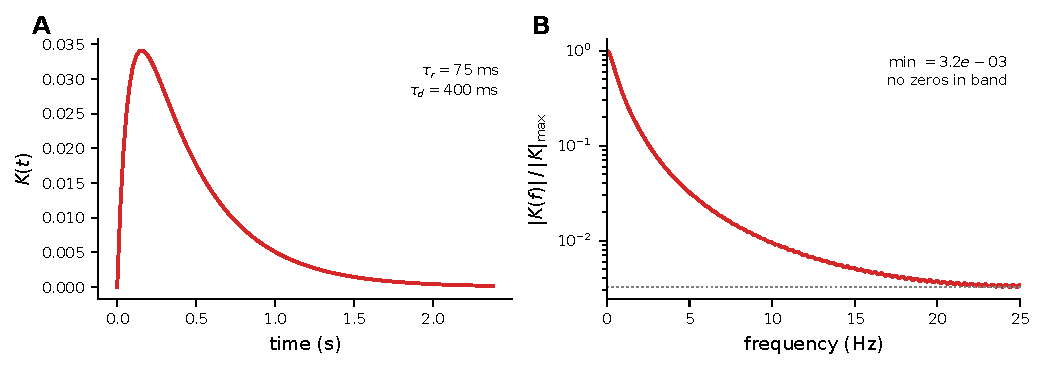
\includegraphics[width=0.82\textwidth]{kernel_fig.pdf}
\caption{The indicator kernel is \emph{given}: the inverse is built from the same
config fields the generator used ($\tau_r$, $\tau_d$, length, $\Delta t$), so $K$
is known exactly rather than estimated. \textbf{A}~$K(t)$, $120$ samples over
$2.4$~s, peak at $0.16$~s, unit sum. \textbf{B}~its transfer function. $|K(f)|$
falls by $308\times$ from DC to Nyquist --- which is why the calcium trace looks
smooth --- but it has \emph{no zeros in band} (minimum
$3.2\times10^{-3}$ of peak, dotted). A convolution with no spectral zeros is
exactly invertible, so the high-frequency content is scaled down, not destroyed.
The worst-case amplification of $308\times$ against float32 precision
($\sim\!10^{-7}$) puts the noise-free error floor near $3\times10^{-5}$, far
below the signal. That is the whole reason panel~C of Fig.~\ref{fig:chain} is
possible, and equally the reason it collapses once photon noise fills the
attenuated band.}
\label{fig:kernel}
\end{figure}

\paragraph{Fitting the raw trace.} With \texttt{observable: calcium} at
$\sigma = 0.05$ the frozen-$W$ regime reappears at every degradation. The oracle,
which fits only the constants of \eqref{eq:gen}, retains partial recovery.

\begin{center}
{\footnotesize
\begin{tabular}{lcccc}
\toprule
& \multicolumn{2}{c}{GNN $\Rw$} & \multicolumn{2}{c}{Known-ODE $\Rw$} \\
\cmidrule(lr){2-3}\cmidrule(lr){4-5}
observable & best & final & best & final \\
\midrule
voltage (control)                 & $0.984$ & $0.983$ & \multicolumn{2}{c}{---} \\
calcium, kernel only              & $-0.010$ & $-0.010$ & $0.373$ & $0.332$ \\
\quad + saturation                & $-0.010$ & $-0.010$ & $0.077$ & $0.006$ \\
\quad + $2$~Hz exposure           & $-0.010$ & $-0.010$ & $0.278$ & $0.277$ \\
\quad + shot noise $\gamma = 0.1$ & $-0.010$ & $-0.010$ & $-0.009$ & $-0.379$ \\
\quad + shot noise $\gamma = 0.2$ & $-0.010$ & $-0.010$ & $-0.009$ & $-0.325$ \\
\quad all composed                & $-0.010$ & $-0.010$ & $-0.009$ & $-0.099$ \\
\bottomrule
\end{tabular}}

{\footnotesize ``best'' = maximum over training, ``final'' = value at $1.52$M
iterations. Both are given because they differ, and the difference is itself a
result (\S2, \emph{decay}). Note that ``best'' for the GNN and for the oracle on
the shot-noise rows is $\approx -0.01$, which is $\widehat{\Mat{W}}$ never leaving
its initialisation: those arms never recovered anything at any point in training,
rather than recovering and then losing it.}
\end{center}

\begin{figure}[t]
\centering
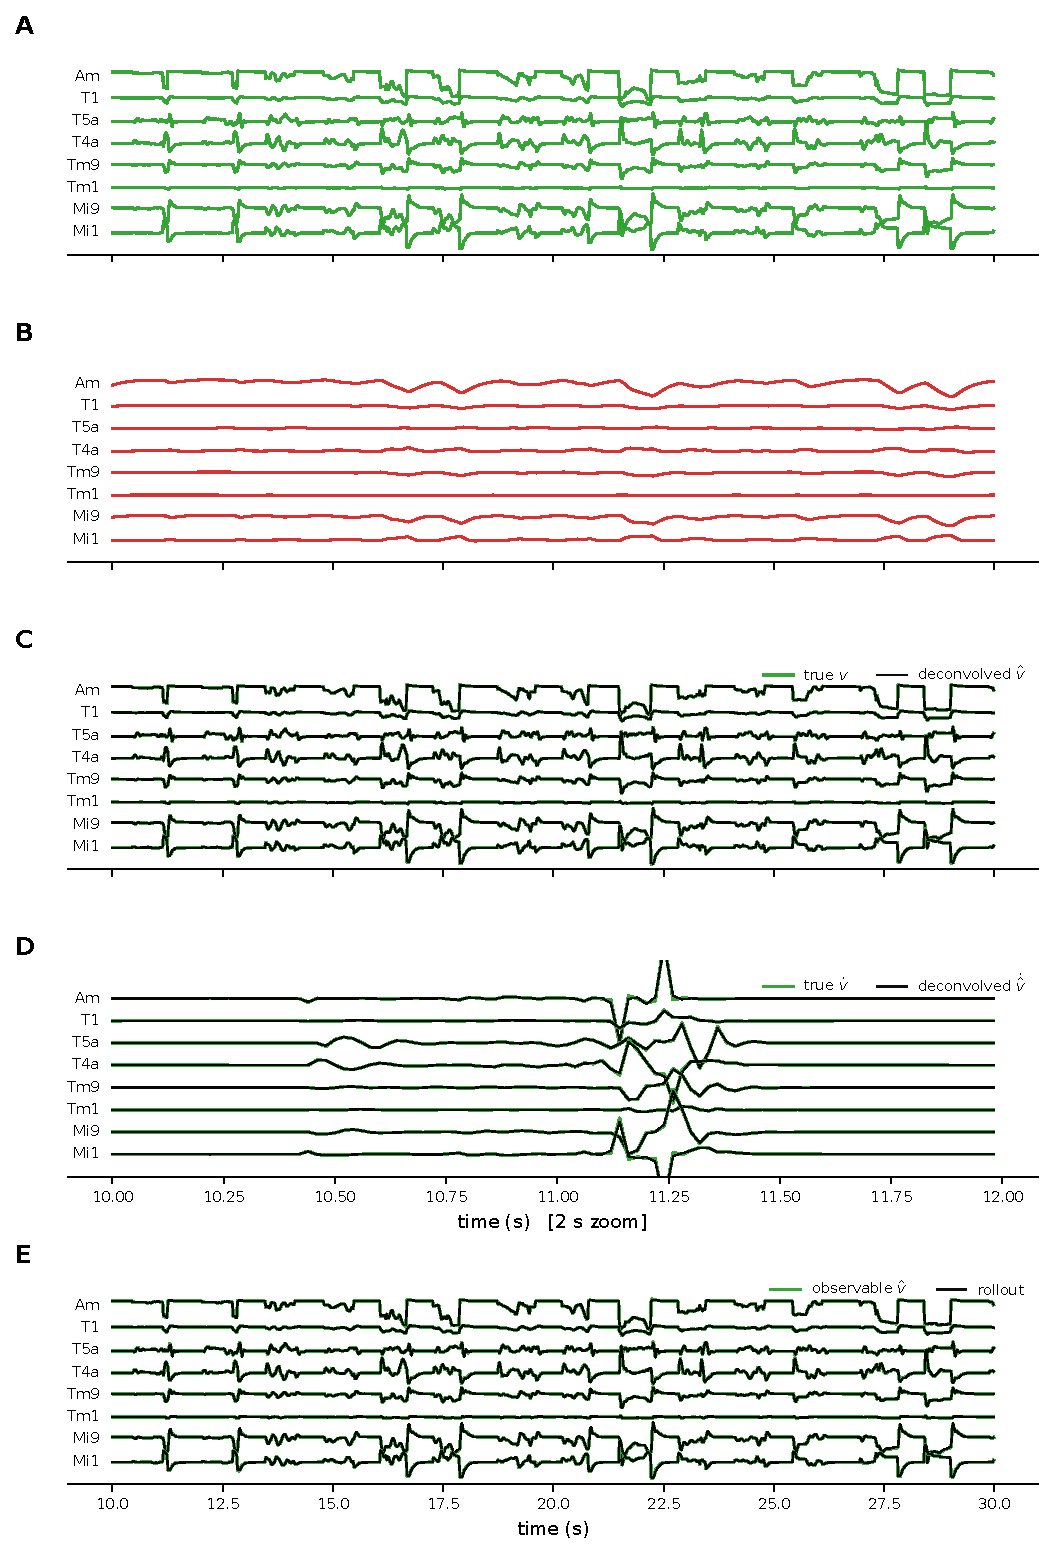
\includegraphics[width=0.86\textwidth]{calcium_fig.pdf}
\caption{The observable chain, no measurement noise, eight reference cell types.
All panels are the same cells over the same held-out test segment, so they can be
read against each other.
\textbf{A}~ground-truth voltage $v$. \textbf{B}~the GCaMP6f observable
$C = K * v$, \emph{same vertical scale}: the fast structure that identifies
$\Mat{W}$ is visibly gone while the slow envelope survives. Quantitatively
$\mathrm{SD}(\dot C) = 0.074\,\mathrm{SD}(\dot v)$, a $13\times$ attenuation ---
but attenuation, not deletion, which is the point, and Fig.~\ref{fig:kernel}B
shows why. \textbf{C}~the Wiener inverse (black) over the truth (green),
$\lambda = 10^{-6}$: $r = 0.9999$. \textbf{D}~the derivative, $2$~s zoom because
at $\Delta t = 20$~ms it is too dense to read over $20$~s; $r(\dot v) = 0.996$.
This is the panel that matters, since $\Mat{W}$ is identified from $\dot v$ and
not from $v$; the deflections here at $11.15$--$11.25$~s are the derivative of
the excursions visible at the same time in A, C and E. \textbf{E}~rollout of the
Known-ODE arm fitted on this observable, $r = 0.9993$. Note the green trace in E
is the \emph{deconvolved observable the model was fitted on}, not the ground
truth, which is the quantity a rollout is scored against; against true voltage it
is also $0.9993$. With a clean trace the chain is lossless end to end; the noise
sweep in the text is what breaks it.}
\label{fig:chain}
\end{figure}

\paragraph{The fix: invert first, then fit.} Deconvolve $C$ back to a voltage
estimate and train an ordinary voltage arm on it, restoring the Markov structure
\eqref{eq:model} assumes (Fig.~\ref{fig:chain}). The inverse is
Tikhonov-regularised in Fourier space,
\begin{equation}
\widehat V(f) = \frac{K^*(f)\,F(f)}{|K(f)|^2 + \lambda\,\max|K|^2\,|R(f)|^2},
\qquad R(f) = \left|1 - e^{-i\omega}\right|^2 .
\label{eq:deconv}
\end{equation}

\paragraph{Deconvolution quality vs.\ photon noise.} $\lambda$ retuned per level
by maximising $r(\dot v)$, so each row is the best inversion available:

\begin{center}
{\footnotesize
\begin{tabular}{lcccc}
\toprule
$\gamma/\mathrm{SD}(C)$ & SNR (dB) & $\lambda$ & $r$ on $v$ & $r$ on $\dot v$ \\
\midrule
$0$    & $\infty$ & $10^{-6}$ & $0.9998$ & $0.993$ \\
$0.01$ & $40.0$   & $10^{-3}$ & $0.980$  & $0.435$ \\
$0.03$ & $30.5$   & $10^{-2}$ & $0.970$  & $0.280$ \\
$0.10$ & $20.0$   & $10^{-1}$ & $0.956$  & $0.172$ \\
\bottomrule
\end{tabular}}
\end{center}

Two-photon GCaMP sits at roughly $20$--$40$~dB, i.e.\ $\gamma/\mathrm{SD} \approx 1$--$10\%$.
The trace stays faithful ($r \geq 0.96$ throughout) while its derivative is
already more than halved at $40$~dB. Since $\Mat{W}$ is read from the derivative,
a high rollout $r$ on a calcium trace is consistent with the weights being
entirely unrecoverable.

\begin{figure}[t]
\centering
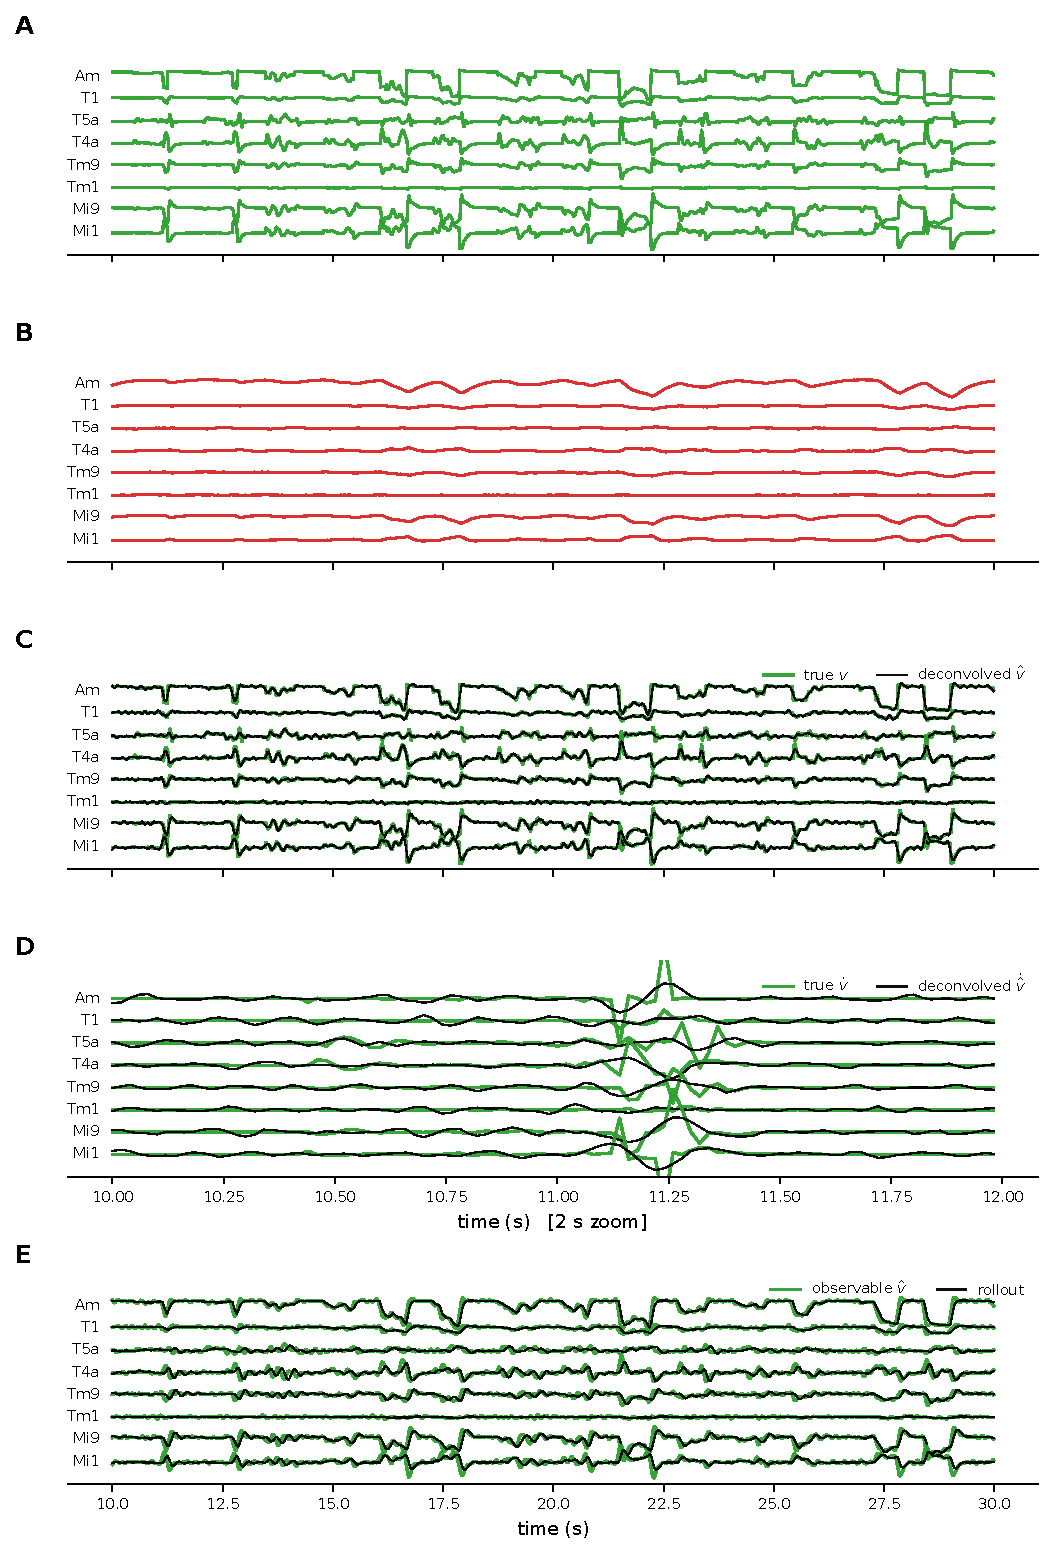
\includegraphics[width=0.86\textwidth]{calcium_fig_g010.pdf}
\caption{The same chain at $\gamma/\mathrm{SD} = 0.01$, i.e.\ $40$~dB --- the
\emph{cleanest} end of the realistic two-photon range. Same cells, same segment,
same panels as Fig.~\ref{fig:chain}, so the two figures can be laid side by side.
Panels A, B, C and E are essentially indistinguishable from the noise-free case:
the calcium trace in B looks the same ($1\%$ noise is invisible at this scale),
the deconvolved voltage in C still tracks the truth at $r = 0.987$, and the
rollout in E is still $r = 0.957$. Panel~D is where the difference is, and it is
not subtle: the deconvolved derivative (black) departs from the truth (green)
everywhere, most visibly across the transient at $11.15$--$11.35$~s, and
$r(\dot v)$ has fallen from $0.996$ to $0.545$. Every panel that an experimenter
would look at to judge the preprocessing still looks right; the one quantity that
$\Mat{W}$ is read from has already lost half its content. This is the figure-level
statement of the whole result, and it is why $\Rw$ collapses at $40$~dB while
rollout $r$ stays high.}
\label{fig:chain40}
\end{figure}

\paragraph{Fits on the deconvolved observable (in progress).}
Eight runs, both arms $\times$ four noise levels. Landed so far:

Eight runs, both arms $\times$ four noise levels. The oracle arms have finished
($1.52$M iterations); the GNN arms are \textbf{still training} and are reported at
$880$k, so their ``final'' column is a running value, not a converged one.

\begin{center}
{\footnotesize
\begin{tabular}{lccccc}
\toprule
& & \multicolumn{2}{c}{GNN $\Rw$ (at $880$k)} & \multicolumn{2}{c}{Known-ODE $\Rw$} \\
\cmidrule(lr){3-4}\cmidrule(lr){5-6}
$\gamma/\mathrm{SD}$ & SNR (dB) & best & current & best & final \\
\midrule
$0$    & $\infty$ & $0.967$  & $0.961$  & $0.915$  & $0.489$ \\
$0.01$ & $40.0$   & $0.144$  & $0.144$  & $0.405$  & $-0.162$ \\
$0.03$ & $30.5$   & $-0.011$ & $-1.234$ & $0.181$  & $-0.159$ \\
$0.10$ & $20.0$   & $-0.010$ & $-0.791$ & $-0.009$ & $-0.142$ \\
\bottomrule
\end{tabular}}
\end{center}

The noise-free row is a \emph{control}, not a result: with a known kernel and no
measurement noise, \eqref{eq:kernel} is exactly invertible and recovering $v$ is
division in Fourier space. A high score there confirms the pipeline; it says
nothing about calcium imaging. The rows that carry the argument are $40$/$30$/$20$~dB,
and there recovery is gone for both arms: the best the oracle reaches at $40$~dB is
$0.405$, and by $20$~dB neither arm ever leaves initialisation.

\paragraph{Decay, and why ``best'' is not free.} On the deconvolved observable the
oracle does not converge --- it peaks early and then drifts away from the truth,
$0.915$ at $32$k falling monotonically to $0.489$ at $1.52$M. This does \emph{not}
happen on true voltage, where oracle runs rise monotonically and end at their
maximum ($0.977$--$0.979$, \texttt{last} $=$ \texttt{max} across five CV folds). The
likely mechanism is that the deconvolved trace is near voltage but not identical
($r = 0.9998$; derivative amplitude $0.93$), and the oracle, having only
$\tau, V^{\mathrm{rest}}, \Mat{W}$ to fit, must absorb that residual mismatch into
$\Mat{W}$; the GNN can absorb it into $f_\theta, g_\phi$ instead and its $\Rw$
plateaus rather than decaying. \emph{This mechanism is inferred from the pattern
and has not yet been measured} --- the direct test is whether the fitted $\tau$ and
$V^{\mathrm{rest}}$ drift in step with the $\Rw$ decay.

Two cautions on the ``best'' columns. Selecting the maximum over training is
early stopping on ground truth, which is unavailable in any real application ---
the same objection the paper raises against its own agentic hyperparameter
search. And at $30$/$20$~dB the GNN also decays (best $-0.011$, current $-1.234$),
so the decay is not unique to the oracle; it is unique to a \emph{misspecified
observable}, and it appears in whichever model lacks the capacity to absorb the
mismatch at that noise level.

\section*{3. Why the first deconvolution failed, and what to fix}

The dataset builder hard-coded $\lambda = 3\times10^{-3}$ with the
\emph{derivative} regulariser. In \eqref{eq:deconv} that sets
$R(f) = |1-e^{-i\omega}|^2$, which is zero at DC and maximal at Nyquist, so the
penalty falls entirely on the high band --- exactly the band $\Mat{W}$ is
identified from. Since $K$ is itself a low-pass, the result is a \emph{double}
low-pass: the indicator attenuated the high frequencies and the regulariser
attenuated them again instead of restoring them. Measured cost: derivative
amplitude $0.28\times$ truth and $r(\dot v) = 0.43$, while $r(v)$ stayed at
$0.98$. The fitted $\Rw = 0.07$ therefore characterised the preprocessing, not
the observation model, and is withdrawn.

The constant came from the figure path, which \emph{injects} synthetic noise when
none is present ($0.20 \times$ per-neuron SD) and then sets $\lambda = 100\sigma^2$.
Heavy smoothing is correct for a noisy trace; the builder copied the constant
while feeding it a clean one.

\paragraph{To fix / to keep fixed.}
\begin{enumerate}\itemsep1pt
\item $\lambda$ must track the noise on the trace, not be a constant. It is now
tuned per level by maximising $r(\dot v)$; $\lambda \approx 10^{-6}$ noise-free.
\item Two edge artefacts must both be handled, and they are different ends. The
FFT is circular, so the end of the record wraps onto its start --- reflect-padding
by one kernel length moves that wrap into discarded material. Separately, frames
$0..3$ are kernel warm-up, where $C$ is an incomplete convolution and $v$ is
genuinely unrecoverable; those are held at the first valid frame. Omitting the
padding alone cost $r(\dot v) = 0.97 \to 0.24$ on the test split.
\item \textbf{Score any deconvolution change on $r(\dot v)$, never on $r(v)$.}
Both defects above were invisible in $r(v)$, which moved by less than $0.02$ while
the derivative lost most of its content.
\item Stimulus discontinuities need no special handling: measured over $800$
abrupt transitions, the error in the following $5$ frames is $1.7\times$ the
median and decays to $1.1\times$ by $20$ frames.
\end{enumerate}

\end{document}
